\documentclass[11pt,a4paper]{article}
\usepackage{amsmath, amsthm, amsfonts, amssymb}
\usepackage{color}
\usepackage{bm}	
\usepackage{float}
\usepackage{caption, subcaption}
\usepackage{times}
\usepackage{fancyhdr}           % Allows better control over headers and footers
%\usepackage{layout}            % use with \layout to see the page layout for
%debugging purposes.
\usepackage[margin=2.5cm]{geometry}  %   set the margins using the
                                %   geometry package (which is much
                                %   the easiest way of doing this).
\usepackage[pdftex]{graphicx}   %   Pictures (means you have to
                                %   produce pdf output via pdflatex)
\usepackage[small,compact]{titlesec}   % Try to reduce the white space
                                % latex loves so much
\titlelabel{\thetitle. \quad}   % Reduce space around section heads
                                % and add a full stop after the number
\pagestyle{fancy}               % Invoke fancy headers

\renewcommand{\abstractname}{\vskip -5mm}  %  Change name of Abstract
                                %  to nothing and loose some of the
                                %  excessive white space
\newcommand{\itab}[1]{\hspace{0em}\rlap{#1}}
\newcommand{\tab}[1]{\hspace{.2\textwidth}\rlap{#1}}

\begin{document}
    \begin{titlepage} \begin{center}
            \textsc{\LARGE University of Cape Town}
            \\[1.5cm] \textsc{\Large Software Engineering Stage Four} \\\smallskip
            \textsc{\Large Final Report} \\\smallskip
            \textsc{\Large CSC3003S} \\\smallskip
            \textsc{\Large \today} \\\smallskip
            \noindent\rule[0.4mm]{\textwidth}{0.1mm}
            \\[0.4cm] { \huge \bfseries Tempest Trace \\[0.4cm] }
            \noindent\rule[0.4mm]{\textwidth}{0.1mm}
            \\[1cm]
            \begin{minipage}[t]{0.4\textwidth}
                \begin{flushleft}\large \emph{Authors:}\\ Brian Mc George - MCGBRI004 \\ Jacques Heunis - HNSJAC003 \\ Timothy Gwynn - GWYTIM001
                    \\[2cm]
                \end{flushleft}
            \end{minipage} \begin{minipage}[t]{0.4\textwidth}
            \begin{flushright} \large \emph{Supervisor:} \\ Assoc. Prof.~Patrick Marais\\patrick@cs.uct.ac.za\end{flushright}
            \begin{flushright} \large \emph{Tutor:} \\ Codie Roelf\\Codie.Roelf@alumni.uct.ac.za\end{flushright}
        \end{minipage}
    \end{center}
\end{titlepage}
\newpage
\tableofcontents
\newpage

%%%  Set the headers via fancyhdr package
\lhead{Capstone Project 2015}  % Short title for running head
\chead{}
\rhead{\today}   %  Fixed running head of the date
\lfoot{}
\cfoot{\thepage}    %  add page number as centre footer.
\rfoot{}
\renewcommand{\headrulewidth}{0.0pt}   % Don't want horizontal line
                                % under header.

\begin{abstract}
 The Tempest Trace project is focused around providing a two player, parkour game. Players race against each other to reach the final goal in a competitive 1st person runner game. Players must move over, under, around and through obstacles efficiently while avoiding enemy AI elements such as flying drones and snipers. An aspect that the game focuses on is allowing the player to choose from a variety of possible routes to gain advantage over his/her opponent; certain routes will be better in different situations so every race requires new strategies.  Players must choose the most efficient route to reach the end goal using their parkour skills ahead of their competitor. The aesthetic is purposefully simplistic and clean to allow the player to focus on gameplay and easily identify obstacles and objects to interact with. Players are also able to interact with the world and each other in order to gain a competitive advantage by slowing their opponent down in a variety of ways. In parkour flow and smoothness of movement are imperative and this is reflected in Tempest Trace, the shortest path is often not the fastest and maintaining movement is often more important than achieving the highest speed.
\end{abstract}

\section{Introduction}
\label{s:introduction}

\section{Requirements Captured}

\section{Design Overview}
\label{s:design-overview}
\subsection{Introduction}
This section outlays the architecture of the system at a class and package level. It also examines the major software patterns that the software adhered to. The system has made use of a number of design patterns to facilitate re-usability and scalability. Specifically the classes relating to the player, since two players are present in the game. As well as the artificial intelligence where there may be several drones or snipers active in the game at a given time. The classes have also been designed to allow tweaking of their internal variables on the fly via the Unity editor. This allows one to make changes to various variables during the game to immediately see the effect the change has on the game. This significantly speeds up the rate at which the game can be balanced and the optimal parameters can be found.
\subsection{Model-View-Controller}
The game can be seen to use a model-view-controller pattern. The benefits of this pattern for the game is that the view of the world is separated from the internal representation of that information. An object's position can be updated in the model and it need not worry about how each player is viewing that object. It helps to maintain consistency as we only update the state once so results in a consistent view on the world for each player. Specifically for games, this pattern holds another advantage; the game back-end can be updated at a rate independent of the rate that the view of the world updates. For example, physics calculations may only be run at 10Hz while the view of the world updates at 60Hz. This allows for better performance management.\smallskip\\
Within the game the models can either be other classes or GameObjects within the game world. The controllers are scripts and classes which send commands to the models to update their state. This state could be a GameObject's position or the current behaviour of a drone for example. The view is what the player sees on the screen. In this game, there are two camera's viewing the world at the same time.
\begin{figure}[H]
    \center{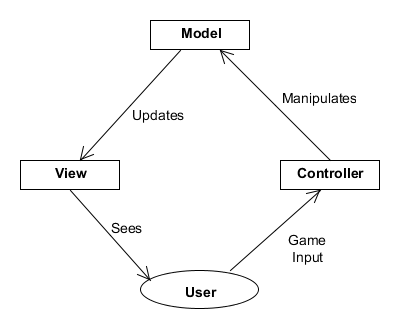
\includegraphics[scale=0.5]{images/MVC.png}}
    \caption{Model-View-Controller within a game context.}
    \label{fig:mvc}
\end{figure}
\subsection{Design class diagram}
The design class digram is too large to fit into an A4 page, it is therefore a separate document: \textit{DesignClassDiagram.pdf}. The class diagram is extensive and highly detailed and shows the relationships between the classes. It also captures the hierarchy between classes. The following is a description of the notation used within the class diagram:
\begin{center}
    \begin{tabular}{|c|c|}
        \hline
        \textbf{Symbol} & \textbf{Description} \\
        \hline
        + & Public \\
        \textasciitilde  & Internal \\
        - & Private \\
        underline & Static \\
        italic & Abstract \\
        \hline
    \end{tabular}    
\end{center}
\subsection{Layered architecture}
The game is build upon the Unity engine. It forms the core or foundation layer of the system. The Unity engine provides functionality for physics calculations, controlling animations, rendering the scene, lighting calculations and collision detection to name a few. No technical services layer was included as the game does not have application-independent services such as connections to databases or extensive logging of errors to file. This layer will be added if in a later iteration a use case that requires such services is developed. The layer above that is the domain layer. It holds software objects representing domain concepts that fulfil application requirements. The majority of the classes belong to this layer since they are specific to the context of this game. At the topmost layer lies the user interface layer. It is highly specific to the application and contains services that the user will interact with. Such services include the world, menus and heads-up display.\smallskip\\
The game makes use of a relaxed layered architecture as the both the user interface layer and domain layer call the engine layer directly. It was decided that a strict layered architecture was inadvisable. The performance impact would be far too high. In a game, the performance is a primary concern. Secondly, it would require a wrapper in the domain layer to allow commands to be passed from the user interface through to the engine layer. \smallskip\\
In this game, the world and level design is a critical factor. It is therefore important to identify where it belongs within the architecture of the system in order to see how changes to it would effect the system as a whole. It was identified that the world should belong to the user interface layer. This is justified as the user can see and interact with the world just as they would see and interact with a web page. The world is therefore classified the same as one would classify the HyperText Markup Language (HTML) and Cascading Style Sheets (CSS) of a web page. The result is that one can make ascetic changes and changes to the layout of the level without affecting any other part of the system.
\begin{figure}[H]
    \center{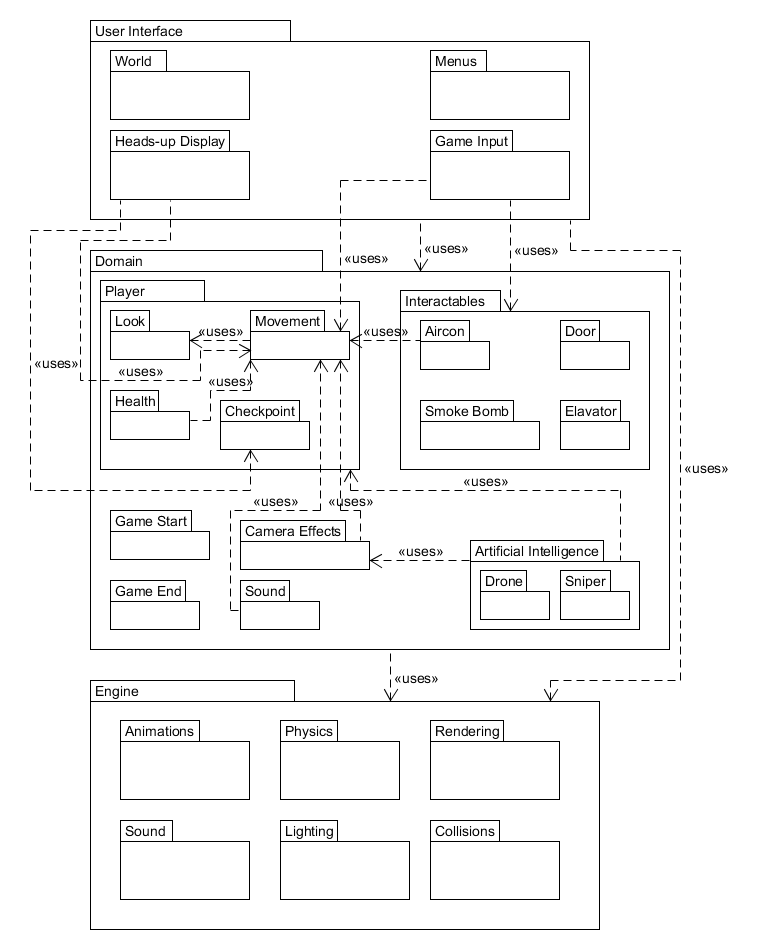
\includegraphics[scale=0.7]{images/LayeredArchitectureDiagram.png}}
    \caption{Architecture of the game}
    \label{fig:architecture}
\end{figure}
\subsection{Data organisation}
The system does not make use of any explicit databases or output to text files. However, since the Unity engine is used it it important to ensure that the data type of the assets used was one which the engine provided support for. The classes were written in C\#, models (possibly with animations) in the fbx format, textures as a png image and materials as a mat file.\smallskip\\
The folder structure of the assets need to be structured and easy to manage to allow the game to scale. A folder for art assets from the artists is used, each assets is then seperated into a different folder. Each folder has the texture, fbx and materials. Fonts, other materials defined, prefabs, scenes, shaders, sound and standard assets are defined to their own folder. A folder called scripts is used to store all the classes. The scripts folder structure is the same as that defined in figure \ref{fig:architecture}.\smallskip\\
The algorithms used will be covered in detail in section \ref{s:implementation} so it will not be covered in this section.

\section{Implementation}
\label{s:implementation}
\subsection{Player Controller}
\subsubsection{Re-usability and Encapsulation}
Since the game must support two independent players, a large amount of code duplication is possible in supporting the interaction of the various game systems with both players. Naturally it is better to avoid code duplication (and in general to stick to the "DRY" - Don't Repeat Yourself - principle) and so extensive use of the engine's built-in object-component model to write instance-independent scripts that will handle the relevant interactions with the world and then simply attach them to the player object. \\
This results in each player object functioning entirely independently, meaning that not only can we simply place an extra player in the world in order to support extra players, but bugs and code modifications only occur once and then the changes simply apply to both players.
\subsubsection{Camera control}
Control of the player's camera is handled by two different scripts, one for rotation in each of the X and Y axes. This separation of axes is useful because while the rotation in the X axis needs to rotate only the camera (and allow the player to look up or down), the rotation about the Y axis also needs to rotate the entire player object (containing the camera, the 3D model, all attached scripts etc). \\
In both the X and Y cases, the script simply gets the relevant player's input for that frame and then rotates itself appropriately.
\subsubsection{Input Separation}
Since our support of multiple players is not over a network and both players must play on the same computer, we need a way to separate the input for either player so that player one does not respond to input intended for player two (for example). This separation is achieved by inserting an extra layer of abstraction between the code that handles player input, and the engine which acquires that input from the operating system/hardware. \\
Instead of asking the engine for the state of input directly, the player scripts ask the "InputSplitter" class for the state of player input for only that player, InputSplitter then handles all separation of input entirely invisibly and only gives back the appropriate commands.
\subsubsection{Environment interaction}
Environment interaction forms the bulk of the code for the player controller. The player needs to be able to compute a number of distinct actions including running, jumping, sliding, climbing and vaulting, all of which require separate handling. Fortunately the transitions between these actions are (in most cases) fairly clear and well-defined, so we use a finite state machine-esque solution. \\
The player's default state is "Idle", where the player is simply standing still and not moving around at all. We can even consider this to be the same state as the player's next most common state: "Running" (since we can think of idling as simply running with a speed of zero). Running is also the state with the most complicated situation regarding state transitions since all the other states transition in and out of Running. \\
While in the Running state, the player can change state either by pressing the jump button, or pressing the slide button. When the slide button is pressed the player will go into a low slide across the ground, as long as they are moving fast enough in the first place. This slide will cause the player to slow down over time (which enforces a limit on how far the player can slide) but will allow them to move beneath low-hanging objects and possibly move around the level in an overall smoother or faster fashion. \\
If the player presses the jump button, the controller first needs to examine the player's surroundings to see what obstacles there are. If there is a low obstacle on the floor in front of the player, then the player will either climb onto it if they are currently stationary, or vault over it if they are moving. If there is an obstacle in front of the player that is too tall to vault over, but not tall enough that the player cannot reach the top of it, then the player will climb up onto the obstacle. If no such obstacles are present, the player will simply jump. \\
In order to facilitate this process of checking the player's surroundings, we make extensive use of the engine's built in physics systems that allow code to easily shoot a ray through the world and provide information about what (if anything) the ray hits. Such a ray cast is used to check for the existence of obstacles at various heights in front of the player, as well as how far upwards those objects extend. \\
\begin{figure}[H]
    \center{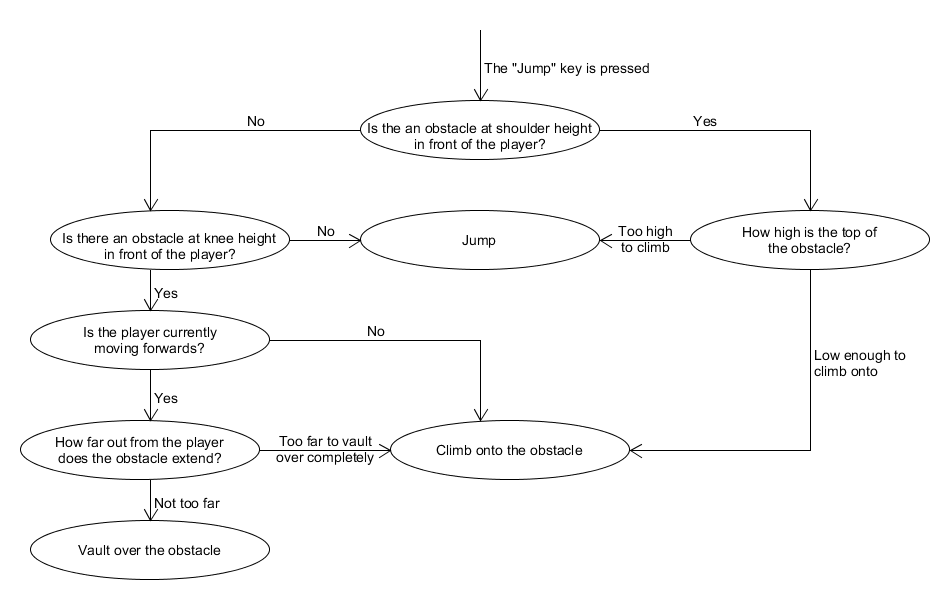
\includegraphics[scale=0.4]{images/JumpDecisionTree.png}}
    \caption{The decision tree that players out when the player presses the "jump" key}
    \label{fig:jumpDecisionTree}
\end{figure}
\subsubsection{Issues encountered}
The main issue encountered while developing the code for controlling the player character is that the code would incorrectly classify the situation when the player pressed the "jump" key and would for example try to climb onto an obstacle that should have been vaulted over. This was mostly caused by badly tuned parameters for deciding at which height obstacles should be checked for, but was also caused by things such as having very thin pieces of world geometry that the system could fail to detect, resulting in incorrect behaviour. \\
The other common issue was that when vaulting, climbing or sliding, the player would clip into world geometry and get stuck. This was a result of those motions failing to correctly make use of the engines physics systems, causing the player to move into geometry and then find themselves stuck when control was returned to the default code for running around. Once again, fixing these issues mostly involved ensuring that the engine's physics state is correctly updated in all the appropriate places while the player is moving.

\section{Program Validation and Verification}
%I Copy-pasted my cases from Stage 3
%This needs to be expanded quite a lot as it does not cover all the cases e.g. missing cases are ones for elevator (ands its interactions with slow button), door, smokebomb (it only has 2 charges!, its interactions with AI), position in the race (UI), the ledge grap, All of AI interactions many possible cases can be thought up there.
\subsubsection{Movement}
\textbf{Tests prepared}\\
Description: Move player forward with no obstruction in the given direction.\\
Expected Result: Player moves forward at the speed configured.\\
Actual Result: As expected.\\
Status: Pass
\smallskip\\
Description: Move player left with no obstruction in the given direction.\\
Expected Result: Player moves left at the speed configured.\\
Actual Result: As expected.\\
Status: Pass
\smallskip\\
Description: Move player right with no obstruction in the given direction.\\
Expected Result: Player moves right at the speed configured.\\
Actual Result: As expected.\\
Status: Pass
\smallskip\\
Description: Move player backwards with no obstruction in the given direction.\\
Expected Result: Player moves backwards at the speed configured.\\
Actual Result: As expected.\\
Status: Pass
\smallskip\\
Description: Move player forwards with an obstruction in the given direction.\\
Expected Result: Player moves forwards at the speed configured until its collider connects with the obstruction, the player can then no longer move forward.\\
Actual Result: As expected.\\
Status: Pass
\smallskip\\
Description: Move player left with an obstruction in the given direction.\\
Expected Result: Player moves left at the speed configured until its collider connects with the obstruction, the player can then no longer move left.\\
Actual Result: As expected.\\
Status: Pass
\smallskip\\
Description: Move player right with an obstruction in the given direction.\\
Expected Result: Player moves right at the speed configured until its collider connects with the obstruction, the player can then no longer move right.\\
Actual Result: As expected.\\
Status: Pass
\smallskip\\
Description: Move player backwards with an obstruction in the given direction.\\
Expected Result: Player moves backwards at the speed configured until its collider connects with the obstruction, the player can then no longer move backwards.\\
Actual Result: As expected.\\
Status: Pass
\smallskip\\
Description: Run animation plays in direction of movement.\\
Expected Result: The run animation plays and makes player model look as if it is running in the given direction\\
Actual Result: No animation plays\\
Status: Failure
\subsubsection{Look}
\textbf{Tests prepared}\\
Description: Player can can turn full 360 degrees horizontally\\
Expected Result: Players view turns horizontally by a configurable angle in the direction of the horizontal mouse movement.\\
Actual Result: As expected.\\
Status: Pass
\smallskip\\
Description: Player can can turn head up to a bounded angle vertically\\
Expected Result: Player view turns vertically by a configurable angle in the direction of the vertical mouse movement. The players vertical view angle is prevented from exceeding the defined range\\
Actual Result: As expected.\\
Status: Pass
\smallskip\\
Description: Player head faces direction of look\\
Expected Result: Player head looks in the direction of the view.\\
Actual Result:  Head remains static.\\
Status: Failure
\subsubsection{Vault}
\textbf{Tests prepared}\\
Description: Player can vault over object that is less than 1 metre high and has a distance that is less than 3 metres and is moving at least 5 metres per second. \\
Expected Result: Player vaults over object.\\
Actual Result:  As expected.\\
Status: Pass
\smallskip\\
Description: Player can not vault over object that is less than 1 metre high and a distance that is more than 3 metres or is moving at less than 5 metres per second. \\
Expected Result: Player climbs onto object.\\
Actual Result:  As expected.\\
Status: Pass
\smallskip\\
Description: Player can not vault over object that is more than 1 metre high\\
Expected Result: Player initiates a climb if it meets the climb parameters else initiates a jump.\\
Actual Result: As expected.\\
Status: Pass
\smallskip\\
Description: Player vault animation plays if vault action initiated\\
Expected Result: The vault animation plays and makes the model look as if it is vaulting over the object.\\
Actual Result:  No animation plays.\\
Status: Failure
\subsubsection{Jump}
\textbf{Tests prepared}\\
Description: The player jumps upwards if no other contextual action available and player is stationary. \\
Expected Result: Player jumps upwards.\\
Actual Result:  As expected.\\
Status: Pass
\smallskip\\
Description: The player jumps in direction of motion if no other contextual action available and player is moving. \\
Expected Result: Player jumps in direction of motion.\\
Actual Result: As expected.\\
Status: Pass
\smallskip\\
Description: The player jump animation plays if player jumps. \\
Expected Result: Jump animation plays.\\
Actual Result:  No animation plays.\\
Status: Failure
\subsubsection{Climb}
\textbf{Tests prepared}\\
Description: The player climbs the object in front of it if it is unable to initiate a vault on the object and it is less than 3.05 metres tall. \\
Expected Result: Player climbs object.\\
Actual Result: As expected.\\
Status: Pass
\smallskip\\
Description: The player climbs animation plays during a climb. \\
Expected Result: Climb animation plays.\\
Actual Result:  No animation plays.\\
Status: Failure
\subsubsection{Slide}
\textbf{Tests prepared}\\
Description: Slide can only be initiated when the player is grounded and is not in a different action\\
Expected Result: Player slides.\\
Actual Result: As expected.\\
Status: Pass
\smallskip\\
Description: Slide decreases player velocity at a defined rate. \\
Expected Result: Player slows down during slide.\\
Actual Result: As expected.\\
Status: Pass
\smallskip\\
Description: Slide can only be initiated if player is moving above a defined amount. \\
Expected Result: Player slides if moving above defined amount. Else, player does not slide\\
Actual Result: As expected.\\
Status: Pass
\smallskip\\
Description: Slide animation plays if a slide is initiated. \\
Expected Result: Player slide animation plays which makes the model look as if it is sliding.\\
Actual Result: No animation plays.\\
Status: Failure
\subsubsection{Re-spawn}
\textbf{Tests prepared}\\
Description: Screen dims when the velocity the player is falling at a defined rate\\
Expected Result: Screen starts to dim.\\
Actual Result: As expected.\\
Status: Pass
\smallskip\\
Description: Screen clears when the velocity the player is not falling at a defined rate\\
Expected Result: Screen starts to clear.\\
Actual Result: As expected.\\
Status: Pass
\smallskip\\
Description: Player re-spawns when the screen dims beyond a defined amount\\
Expected Result: Player re-spawns at last checkpoint reached and screen clears.\\
Actual Result: As expected.\\
Status: Pass
\subsubsection{Checkpoints}
\textbf{Tests prepared}\\
Description: Latest checkpoint updates if the players reaches a checkpoint not in set of checkpoints reached.\\
Expected Result: Latest checkpoint set as the current checkpoint reached.\\
Actual Result: As expected.\\
Status: Pass
\smallskip\\
Description: Latest checkpoint does not update if the players reaches a checkpoint already in set of checkpoints reached.\\
Expected Result: No change to system.\\
Actual Result: As expected.\\
Status: Pass

\subsection{Environment}
\subsubsection{Aircon vent expels steam to slow player}
\textbf{Tests prepared}\\
Description: Player only slowed when the aircon is active.\\
Expected Result: Player is slowed.\\
Actual Result: As expected.\\
Status: Pass
\smallskip\\
Description: Steam only shows if aircon is active.\\
Expected Result: Steam effect expelled from aircon vent.\\
Actual Result: As expected.\\
Status: Pass
\smallskip\\
Description: Player is not slowed when the aircon is not active.\\
Expected Result: Player is not slowed.\\
Actual Result: As expected.\\
Status: Pass
\section{Conclusion}

\newpage
\section*{User Manual}
\label{ss:user-manual}
\begin{description}
	\item [Goal] Get to the top of the last building before the other player. Move quickly and efficiently while avoiding danger from enemies and falls.
	\item [Enemies] Flying drones will attempt to chase you down if you get too close to them. Snipers will shoot you if you expose yourself in their field of vision.
	\item [Environment] Interact with objects such as doors and buttons in your environment by pressing the object interaction button. Buttons will often let you gain a tactical advantage over your opponent.
	\item [Player 1 Controls]\hfill \\
	\begin{description}
		\item \itab{Look:}\tab{Mouse}
		\item \itab{Movement:}\tab{WASD}
		\item \itab{Jump:}\tab{Spacebar}
		\item \itab{Slide:}\tab{Shift}
		\item \itab{Somkebomb:}\tab{F}
		\item \itab{Object Interaction:}\tab{E}
	\end{description}
	\item [Player 2 Controls]\hfill \\
	\begin{description}
		\item \itab{Look:}\tab{Right Joystick}
		\item \itab{Movement:}\tab{Left Joystick}
		\item \itab{Jump:}\tab{Left Bumper}
		\item \itab{Slide:}\tab{Right Bumper}
		\item \itab{Somkebomb:}\tab{B Button}
		\item \itab{Object Interaction:}\tab{A Button}
	\end{description}
\end{description}
\newpage
\begin{thebibliography}{9}

\bibitem[Kopka and Daly(2004)]{KopkaDaly}
Kopka, H. and Daly, P.W.  (2004) \textit{A Guide to \LaTeXe:
Document Preparation for Beginners and Advanced Users} (4th~edn).
Addison-Wesley.

\bibitem[Lamport(1994)]{Lamport}
Lamport L. (1994) \textit{\LaTeX: A Document Preparation System}
(2nd~edn). Addison-Wesley.

\bibitem[Mittelbach and Goossens(2004)]{Companion}
Mittelbach, F. and Goossens, M., (2004) \textit{The \LaTeX\
Companion} (2nd~edn). Addison-Wesley.
\end{thebibliography}
\end{document}
